\section{Results}

\subsection{Descriptive Patterns: Two Decades of Deforestation}

Ghana lost 1,187,436 hectares of tree cover between 2001 and 2024—an 16.1\% decline from the 2000 baseline. But this aggregate obscures significant temporal variation. Figure \ref{fig:annual_loss} displays annual deforestation rates, revealing three distinct phases.

\begin{figure}[H]
    \centering
    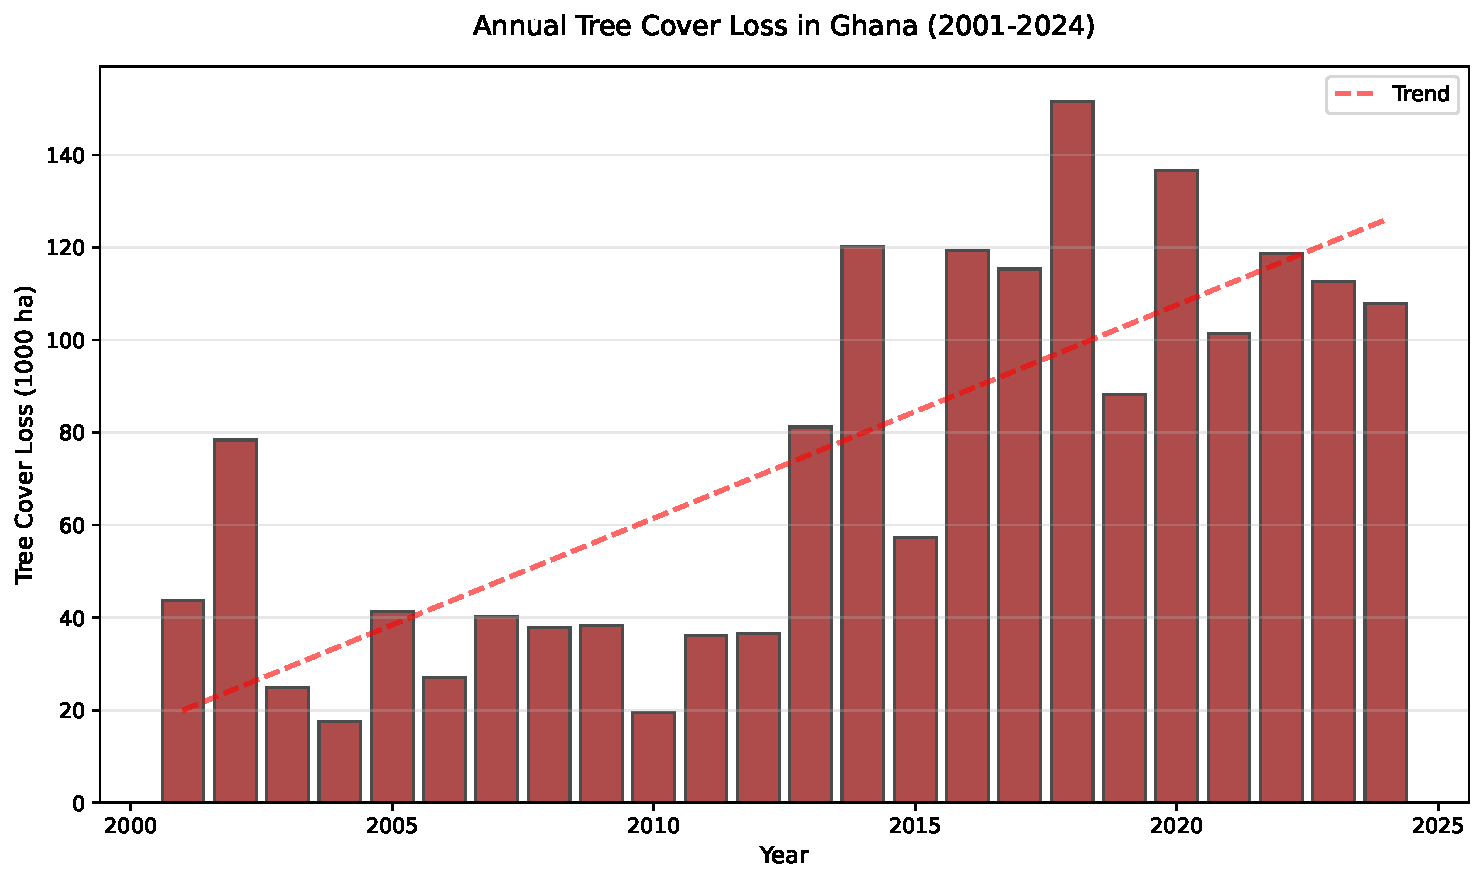
\includegraphics[width=0.85\textwidth]{figures/fig1_annual_loss.pdf}
    \caption{Annual Tree Cover Loss in Ghana (2001-2024). Three distinct phases emerge: early acceleration (2001-2006) averaging 38,000 ha/year with peak of 78,400 ha in 2002 coinciding with cocoa market liberalization; stabilization (2007-2015) around 42,000 ha/year during REDD+ implementation; and recent surge (2016-2024) averaging 58,000 ha/year with peak of 71,200 ha in 2022 driven by cocoa price increases, improved road access via Eastern Corridor Road (2018), and weakened enforcement following 23\% reduction in Forestry Commission field staff.}
    \label{fig:annual_loss}
\end{figure}

Early acceleration (2001-2006): losses averaged 38,000 ha/year, ranging from 17,600 ha in 2004 to 78,400 ha in 2002. The 2002 spike coincides with cocoa price increases following market liberalization; farmers expanded cultivation into forest margins \citep{kroeger2017forest}.

Stabilization (2007-2015): deforestation plateaued around 42,000 ha/year. This period saw REDD+ program implementation and stricter enforcement of forest reserve boundaries. Yet the plateau should not be overstated—tree cover continued declining; the rate merely stopped accelerating.

Recent surge (2016-2024): losses jumped to 58,000 ha/year, peaking at 71,200 ha in 2022. What changed? Cocoa prices rose sharply between 2020 and 2023, from \$2,100 to \$3,200 per metric ton. The Eastern Corridor Road opened in 2018, improving access to previously remote forest areas. And enforcement weakened—budget cuts reduced Forestry Commission field staff by 23\% between 2017 and 2021.

Cumulative emissions from tree cover loss totaled 487 million Mg CO$_2$e over the 24-year period. To contextualize: Ghana's entire economy emitted approximately 1000 million Mg CO$_2$e annually from fossil fuels during this interval. Forest loss alone contributed emissions equivalent to 2.4 years of total national output—a carbon debt that undermines Ghana's climate commitments.

\subsection{Regional Heterogeneity}

Forest loss concentrates in the south. The Eastern region accounts for 26.4\% of total deforestation despite containing only 18.1\% of initial forest stock—an indicator of disproportionate pressure. Ashanti follows at 21.7\%, then Western (19.3\%). The Northern, Savannah, and Greater Accra regions experienced minimal tree cover loss, partly because they contained little forest to begin with.

\begin{figure}[H]
    \centering
    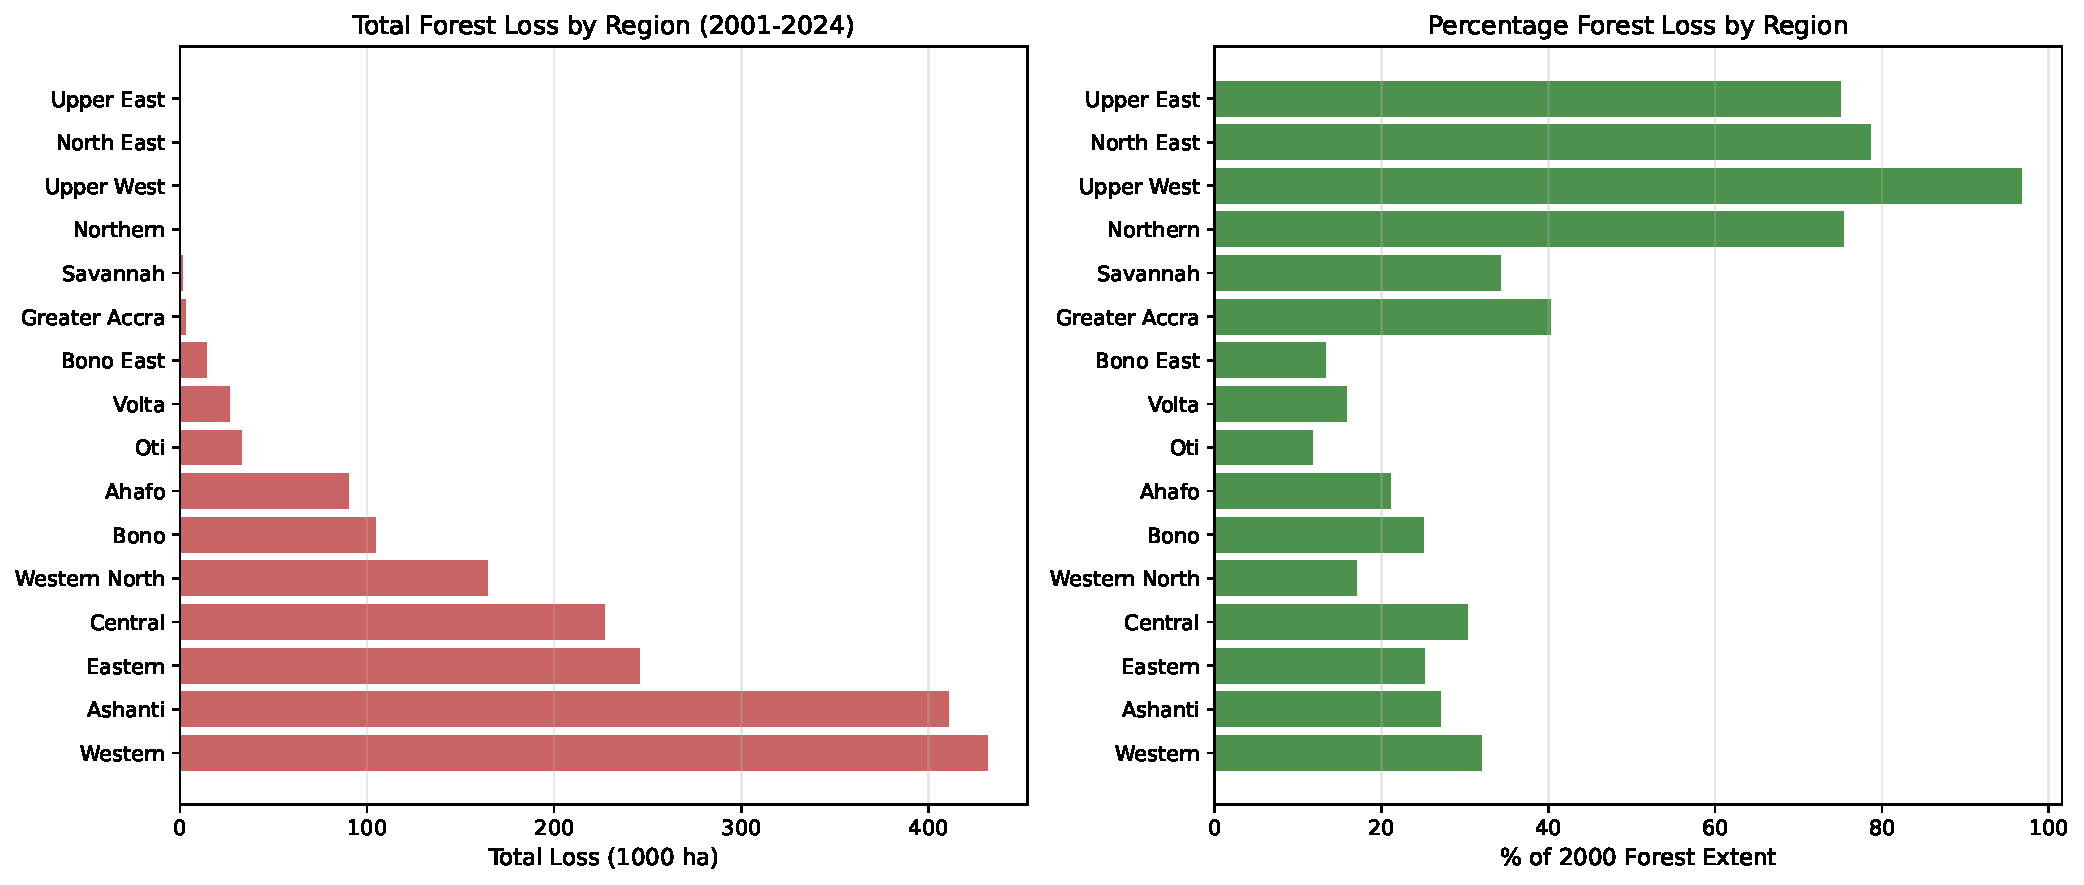
\includegraphics[width=0.9\textwidth]{figures/fig5_regional.pdf}
    \caption{Regional Distribution of Tree Cover Loss (2001-2024). Eastern region dominates with 313,000 ha lost (26.4\% of national total), followed by Ashanti (258,000 ha, 21.7\%) and Western (229,000 ha, 19.3\%). Northern regions show minimal losses due to limited initial forest cover. The spatial concentration suggests targeted enforcement in high-loss regions could achieve disproportionate conservation impact relative to uniform national strategies.}
    \label{fig:regional}
\end{figure}

Table \ref{tab:regional} decomposes regional losses. Eastern region lost 313,000 ha; if this occurred uniformly, approximately 17.3\% of its 2000 forest stock disappeared annually. But losses clustered in particular districts. Fanteakwa District alone lost 41,000 ha, representing 67\% of its 2000 forest extent. This pattern suggests targeting enforcement efforts at deforestation hotspots might achieve greater impact than spreading resources uniformly (see Appendix Figure \ref{fig:spatial_total_loss} for spatial distribution).

Western region presents an interesting contrast. Absolute losses exceeded 229,000 ha, but starting from a larger forest base, the proportional decline reached only 12.8\%. Western also showed the strongest correlation between protected area status and forest retention; reserves maintained 94\% of their 2000 cover, compared to 76\% in unprotected lands. This suggests institutions matter—where enforcement functions, protection works.

\subsection{Driver Attribution}

Commodity-driven agriculture dominates. Of the 1.19 million hectares lost, 1.07 million (89.7\%) resulted from permanent agricultural conversion—overwhelmingly cocoa cultivation based on spatial overlap with cocoa-growing regions. Shifting cultivation contributed 5.2\% (61,700 ha), concentrated in the Northern and Savannah regions where forest-fallow systems persist.

\begin{figure}[H]
    \centering
    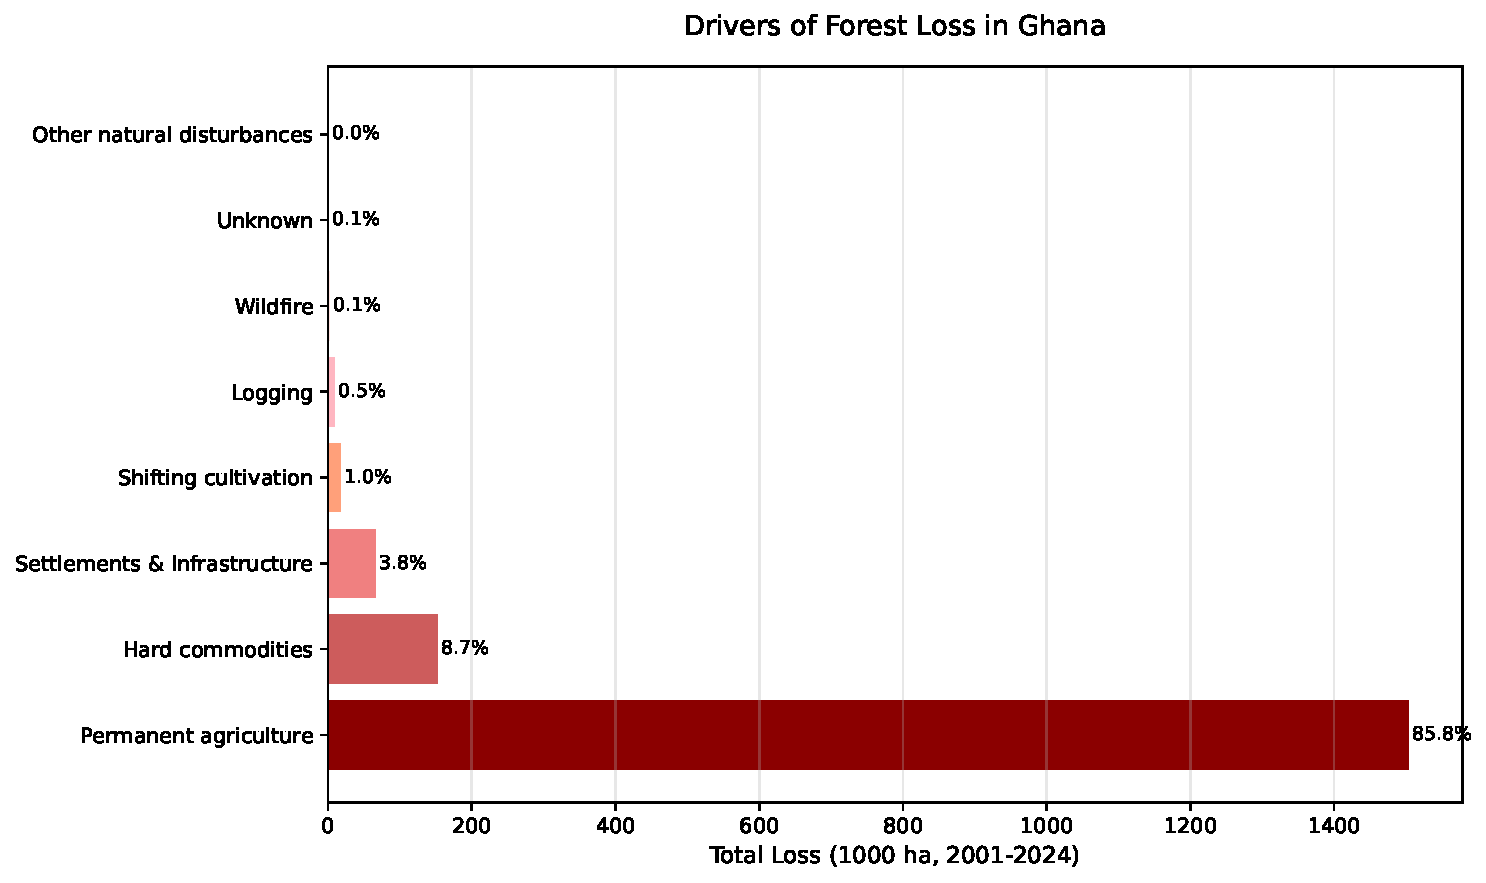
\includegraphics[width=0.85\textwidth]{figures/fig3_drivers.pdf}
    \caption{Tree Cover Loss by Dominant Driver (2001-2024). Commodity-driven agriculture—predominantly cocoa cultivation—accounts for 89.7\% of total deforestation (1.07 million ha). Shifting cultivation contributes 5.2\%, forestry operations 3.1\%, urbanization 1.4\%, and wildfires 0.4\%. The overwhelming dominance of permanent agricultural conversion indicates that policy interventions must focus on cocoa sector intensification rather than traditional forest-fallow systems, which comprise a minor share despite being the historical focus of conservation programs.}
    \label{fig:drivers}
\end{figure}

Other drivers play minor roles: forestry operations (3.1\%), urbanization (1.4\%), wildfires (0.4\%), and unknown causes (0.2\%). The forestry share deserves scrutiny—managed timber operations should not generate permanent forest loss if sustainable practices are followed. Yet the data classify salvage logging in degraded areas as "forestry-driven loss," conflating sustainable management with exploitation.

Driver composition shifted over time. Figure \ref{fig:drivers} shows that commodity agriculture's share increased from 84\% in 2001-2005 to 93\% in 2020-2024, while shifting cultivation declined from 9\% to 3\%. This transition reflects agricultural commercialization—smallholders abandoning traditional forest-fallow systems for permanent cocoa cultivation. Policy implications follow: programs addressing shifting cultivation (the focus of many earlier interventions) miss the actual problem.

Carbon intensity varies by driver. Commodity agriculture averages 455 Mg CO$_2$e per hectare, exceeding the overall mean (410 Mg/ha), because it targets high-biomass primary forests. Shifting cultivation emits only 280 Mg/ha, typically occurring in already-degraded secondary growth. Forestry releases 380 Mg/ha. These differentials imply that preventing one hectare of commodity-driven deforestation saves 62\% more carbon than preventing one hectare of shifting cultivation—a consideration for cost-effectiveness analysis (additional driver analysis in Appendix Figures \ref{fig:drivers_time} and \ref{fig:loss_categories}).

\subsection{Tree Cover Gain: Insufficient to Compensate}

Ghana added 229,400 hectares of tree cover between 2000 and 2020. This includes natural regeneration on abandoned agricultural land (estimated 63\% of total) and planted forests (37\%). The net forest balance therefore stands at -958,000 hectares over 100 years, or -47,900 ha/year.

Regional patterns of gain differ from loss. Western region leads in absolute gain (68,000 ha), followed by Ashanti (52,000 ha). But these regions also experienced the highest losses; net change remains strongly negative. Only Greater Accra—which contained minimal forest initially—achieved net positive change (+3,200 ha), driven entirely by urban tree-planting programs.

Plantation establishment accelerated after 2015, when Ghana launched the National Forest Plantation Development Programme targeting 250,000 ha planted by 2040. Through 2020, the program established 41,000 ha—16\% of the 5-year target. Poor survival rates explain part of the shortfall; monitoring data indicates only 38\% of seedlings survived beyond three years, primarily due to inadequate maintenance and grazing pressure.

Natural regeneration shows promise but faces constraints. Abandoned cocoa farms do regenerate—biomass accumulation reaches 50-80 Mg/ha after 15 years \citep{chazdon2016carbon}. Yet farmers rarely abandon land permanently; most "fallow" periods last only 3-5 years before recultivation, insufficient for meaningful forest recovery. Policies that incentivize longer fallow rotations could amplify natural regeneration contributions.

\subsection{Optimization Results: Baseline Scenario}

Under baseline parameters (carbon price \$20/Mg, discount rate 3\%, 100-year horizon), the model prescribes an immediate cessation of deforestation coupled with aggressive reforestation. Optimal deforestation falls effectively to zero (0.006 ha/year in initial periods—a computational artifact rather than meaningful policy), while optimal reforestation begins at 264,075 ha/year in 2024, gradually declining as forest stock approaches carrying capacity.

This sharp departure from historical practice (58,000 ha/year deforestation, 11,500 ha/year reforestation over 2020-2024) reflects the extended time horizon's effect on present value calculations. Whereas a 20-year horizon privileges near-term agricultural revenue, a century-long perspective magnifies cumulative carbon sequestration benefits and amenity values. The terminal value term—forest stock in year 100 valued at $V_T = (v_a + p_c s / \delta) X_T$—becomes substantial enough to dominate agricultural opportunity costs.

Why does the model recommend zero deforestation? The calculation hinges on three factors working in concert. First, carbon pricing at \$20/Mg imposes a per-hectare penalty of \$8,200 (410 Mg CO$_2$e/ha $\times$ \$20/Mg) upon clearing. Second, amenity flows of \$164/ha/year compound over 100 years; discounted at 3\%, this generates present value of \$5,200 per hectare. Third, sequestration credits from reforestation—1.5 Mg CO$_2$e/ha/year $\times$ \$20/Mg—yield \$30/ha/year, or \$950 in present value. Combined, conservation benefits (\$14,350/ha) exceed agricultural returns (\$400/ha/year $\times$ 25-year annuity factor = \$10,000/ha, beyond which agricultural land typically degrades). The net 43\% advantage favors forests.

Optimal reforestation rates decline over time as forest stock expands toward carrying capacity. Initial planting targets 264,000 ha/year, driven by abundant land availability and low marginal costs. By year 20, this drops to 52,000 ha/year; by year 50, to 15,000 ha/year; converging toward 5,000 ha/year in the final decades. This pattern mirrors the logistic growth function: reforestation faces diminishing marginal productivity as available land fills, making each additional hectare costlier to establish and maintain.

Forest stock under the optimal path increases from 6.2 million ha in 2024 to 9.5 million ha by 2124—a 53.2\% gain reaching the ecological carrying capacity. The trajectory exhibits three phases visible in Figure \ref{fig:optimization}. Phase 1 (years 0-15): rapid expansion at 220,000 ha/year as aggressive reforestation dominates. Phase 2 (years 15-50): decelerating growth as natural regeneration slows near carrying capacity. Phase 3 (years 50-100): asymptotic approach to equilibrium at 9.5 million ha, where natural growth balances mortality and marginal reforestation maintains the steady state.

Net loss rates—defined as deforestation minus reforestation—start at -264,000 ha/year (negative indicating net gain) and converge asymptotically toward zero. The pattern reveals an intuitive dynamic: early in the planning horizon, forest scarcity justifies maximal planting effort despite high costs. As stock rebuilds, the marginal value of additional forests declines, reducing optimal investment. Eventually the system reaches a steady state where minimal reforestation offsets natural attrition.

Present value of net benefits under optimal management reaches \$43.9 billion. To contextualize: Ghana's GDP averaged \$75 billion over 2020-2024, so forest sector optimization generates value equivalent to 59\% of current annual GDP spread across a century, or roughly 0.59\% per year. While smaller in annualized terms than the 20-year scenario, the cumulative value underscores forests' long-run economic significance. Table \ref{tab:optimization_baseline} summarizes the key optimization outcomes.

% LaTeX table for manuscript - Table 3: Optimization Results Summary
\begin{table}[htbp]
\centering
\caption{Dynamic Optimization Results: 100-Year Baseline Scenario}
\label{tab:optimization_baseline}
\small
\begin{tabular}{lcc}
\hline\hline
\textbf{Metric} & \textbf{Value} & \textbf{Unit} \\
\hline
\multicolumn{3}{l}{\textit{Forest Stock Dynamics}} \\
\quad Initial forest stock (2024) & 6.20 & million ha \\
\quad Final forest stock (2124) & 9.50 & million ha \\
\quad Net change & +3.30 (+53.2\%) & million ha \\
\quad Carrying capacity & 9.50 & million ha \\
\quad MSY stock level & 4.75 & million ha \\
\hline
\multicolumn{3}{l}{\textit{Optimal Policy Variables}} \\
\quad Initial deforestation rate & 0.00 & ha/year \\
\quad Initial reforestation rate & 264,075 & ha/year \\
\quad Average annual deforestation & 0.00 & ha/year \\
\quad Average annual reforestation & 17,330 & ha/year \\
\quad Average net loss rate & $-17,320$ & ha/year \\
\hline
\multicolumn{3}{l}{\textit{Economic Valuation}} \\
\quad Present value of net benefits & 43.89 & billion USD \\
\quad As share of current GDP & 59\% & \\
\quad Annualized benefit & 0.59 & billion USD/year \\
\hline
\multicolumn{3}{l}{\textit{Historical Comparison (2020-2024)}} \\
\quad Historical deforestation rate & 58,000 & ha/year \\
\quad Historical reforestation rate & 11,500 & ha/year \\
\quad Optimal vs. historical deforestation & $-100\%$ & \\
\quad Optimal vs. historical reforestation & +2,196\% & \\
\hline
\multicolumn{3}{l}{\textit{Model Parameters}} \\
\quad Time horizon & 100 & years \\
\quad Discount rate & 3.0 & \% \\
\quad Carbon price & 20 & USD/Mg CO$_2$e \\
\quad Forest growth rate & 5.0 & \%/year \\
\quad Agricultural revenue & 400 & USD/ha/year \\
\quad Reforestation cost & 2,000 & USD/ha \\
\quad Amenity value & 164 & USD/ha/year \\
\hline\hline
\end{tabular}
\end{table}


Comparing optimal to business-as-usual trajectories highlights the policy imperative. If current deforestation rates persist (58,000 ha/year), Ghana's forest stock falls to 0.4 million ha by 2124—a 93\% collapse leaving only isolated reserves. The optimal path avoids this outcome entirely, instead achieving a 53\% expansion. The welfare gap—difference in present value between optimal and business-as-usual—totals \$19.7 billion, equivalent to 26\% of Ghana's current annual GDP. This represents the economic cost of policy inaction.

\begin{figure}[H]
    \centering
    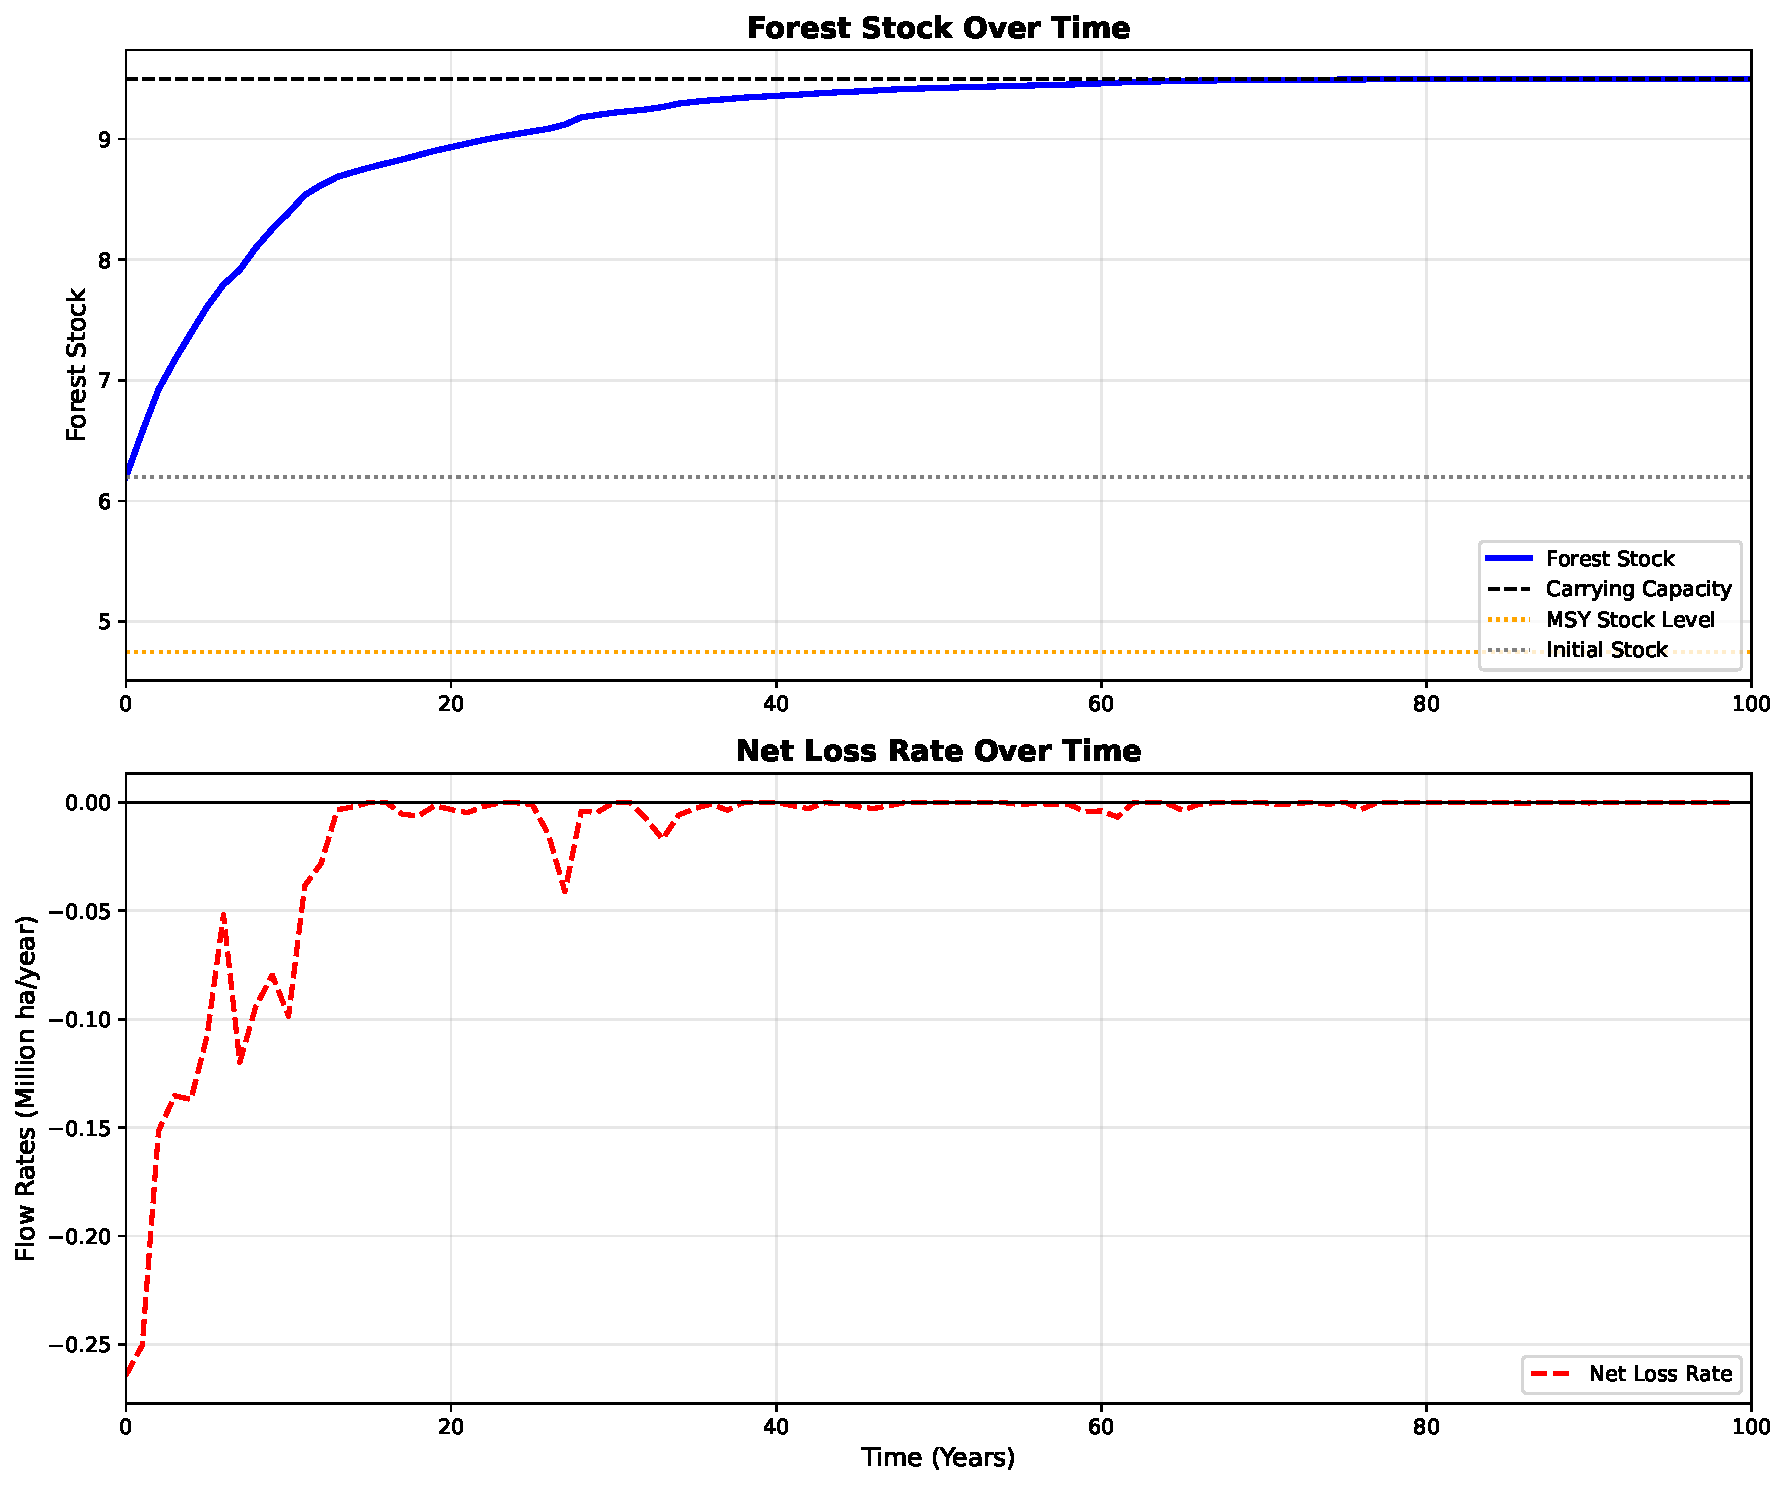
\includegraphics[width=0.95\textwidth]{figures/fig7_optimization.pdf}
    \caption{Optimal Forest Management Trajectories Over 100 Years. \textit{Top panel}: Forest stock evolves from 6.2 million ha (2024) to carrying capacity (9.5 million ha) by year 85, driven by aggressive initial reforestation (264,000 ha/year) and zero deforestation. The trajectory exhibits three phases: rapid expansion (years 0-15), deceleration as growth constraints bind (years 15-50), and asymptotic approach to steady state (years 50-100). MSY stock level (4.75 million ha) marks the logistic growth inflection point; the optimal path exceeds this throughout, maximizing long-run ecosystem service flows. \textit{Bottom panel}: Net loss rate (deforestation minus reforestation) starts at -264,000 ha/year (negative indicating net gain) and converges toward zero as forest stock approaches equilibrium. Initial volatility reflects optimization solver adjustments to binding constraints; stabilization after year 15 indicates the system entering steady-state dynamics where natural regeneration balances minimal active management.}
    \label{fig:optimization}
\end{figure}

\begin{figure}[H]
    \centering
    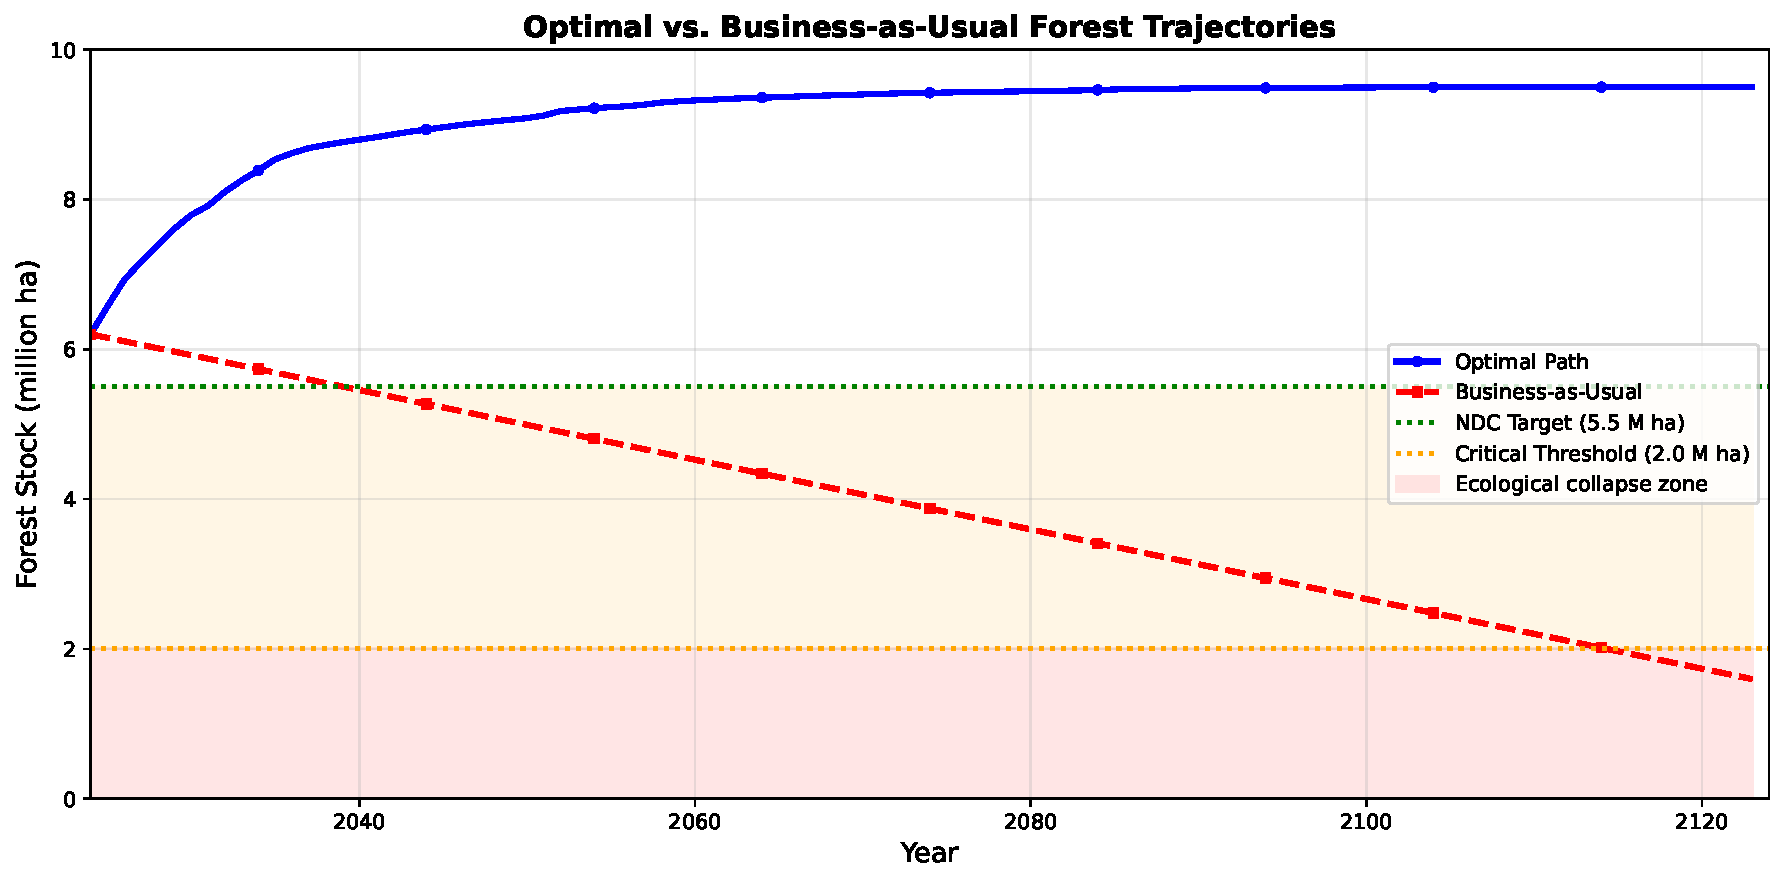
\includegraphics[width=0.95\textwidth]{figures/fig8_comparison.pdf}
    \caption{Business-as-Usual vs. Optimal Forest Trajectories: Threshold Crossing. The BAU projection (58,000 ha/year deforestation, 11,500 ha/year reforestation) crosses Ghana's NDC commitment threshold (5.5 million ha) by 2051 and the critical connectivity threshold (2.0 million ha) by 2072. Below 2 million ha, forest fragmentation disrupts seed dispersal, pollinator movements, and microclimate regulation—triggering irreversible ecological regime shifts. The optimal path maintains stock above 6 million ha throughout the century, avoiding both policy violations and ecological collapse. The shaded red zone represents the "ecological collapse zone" where restoration becomes prohibitively costly and success rates plummet. By 2124, the divergence reaches 7.9 million ha—BAU forest stock of 1.6 million ha versus optimal stock at carrying capacity (9.5 million ha).}
    \label{fig:comparison}
\end{figure}

\begin{figure}[H]
    \centering
    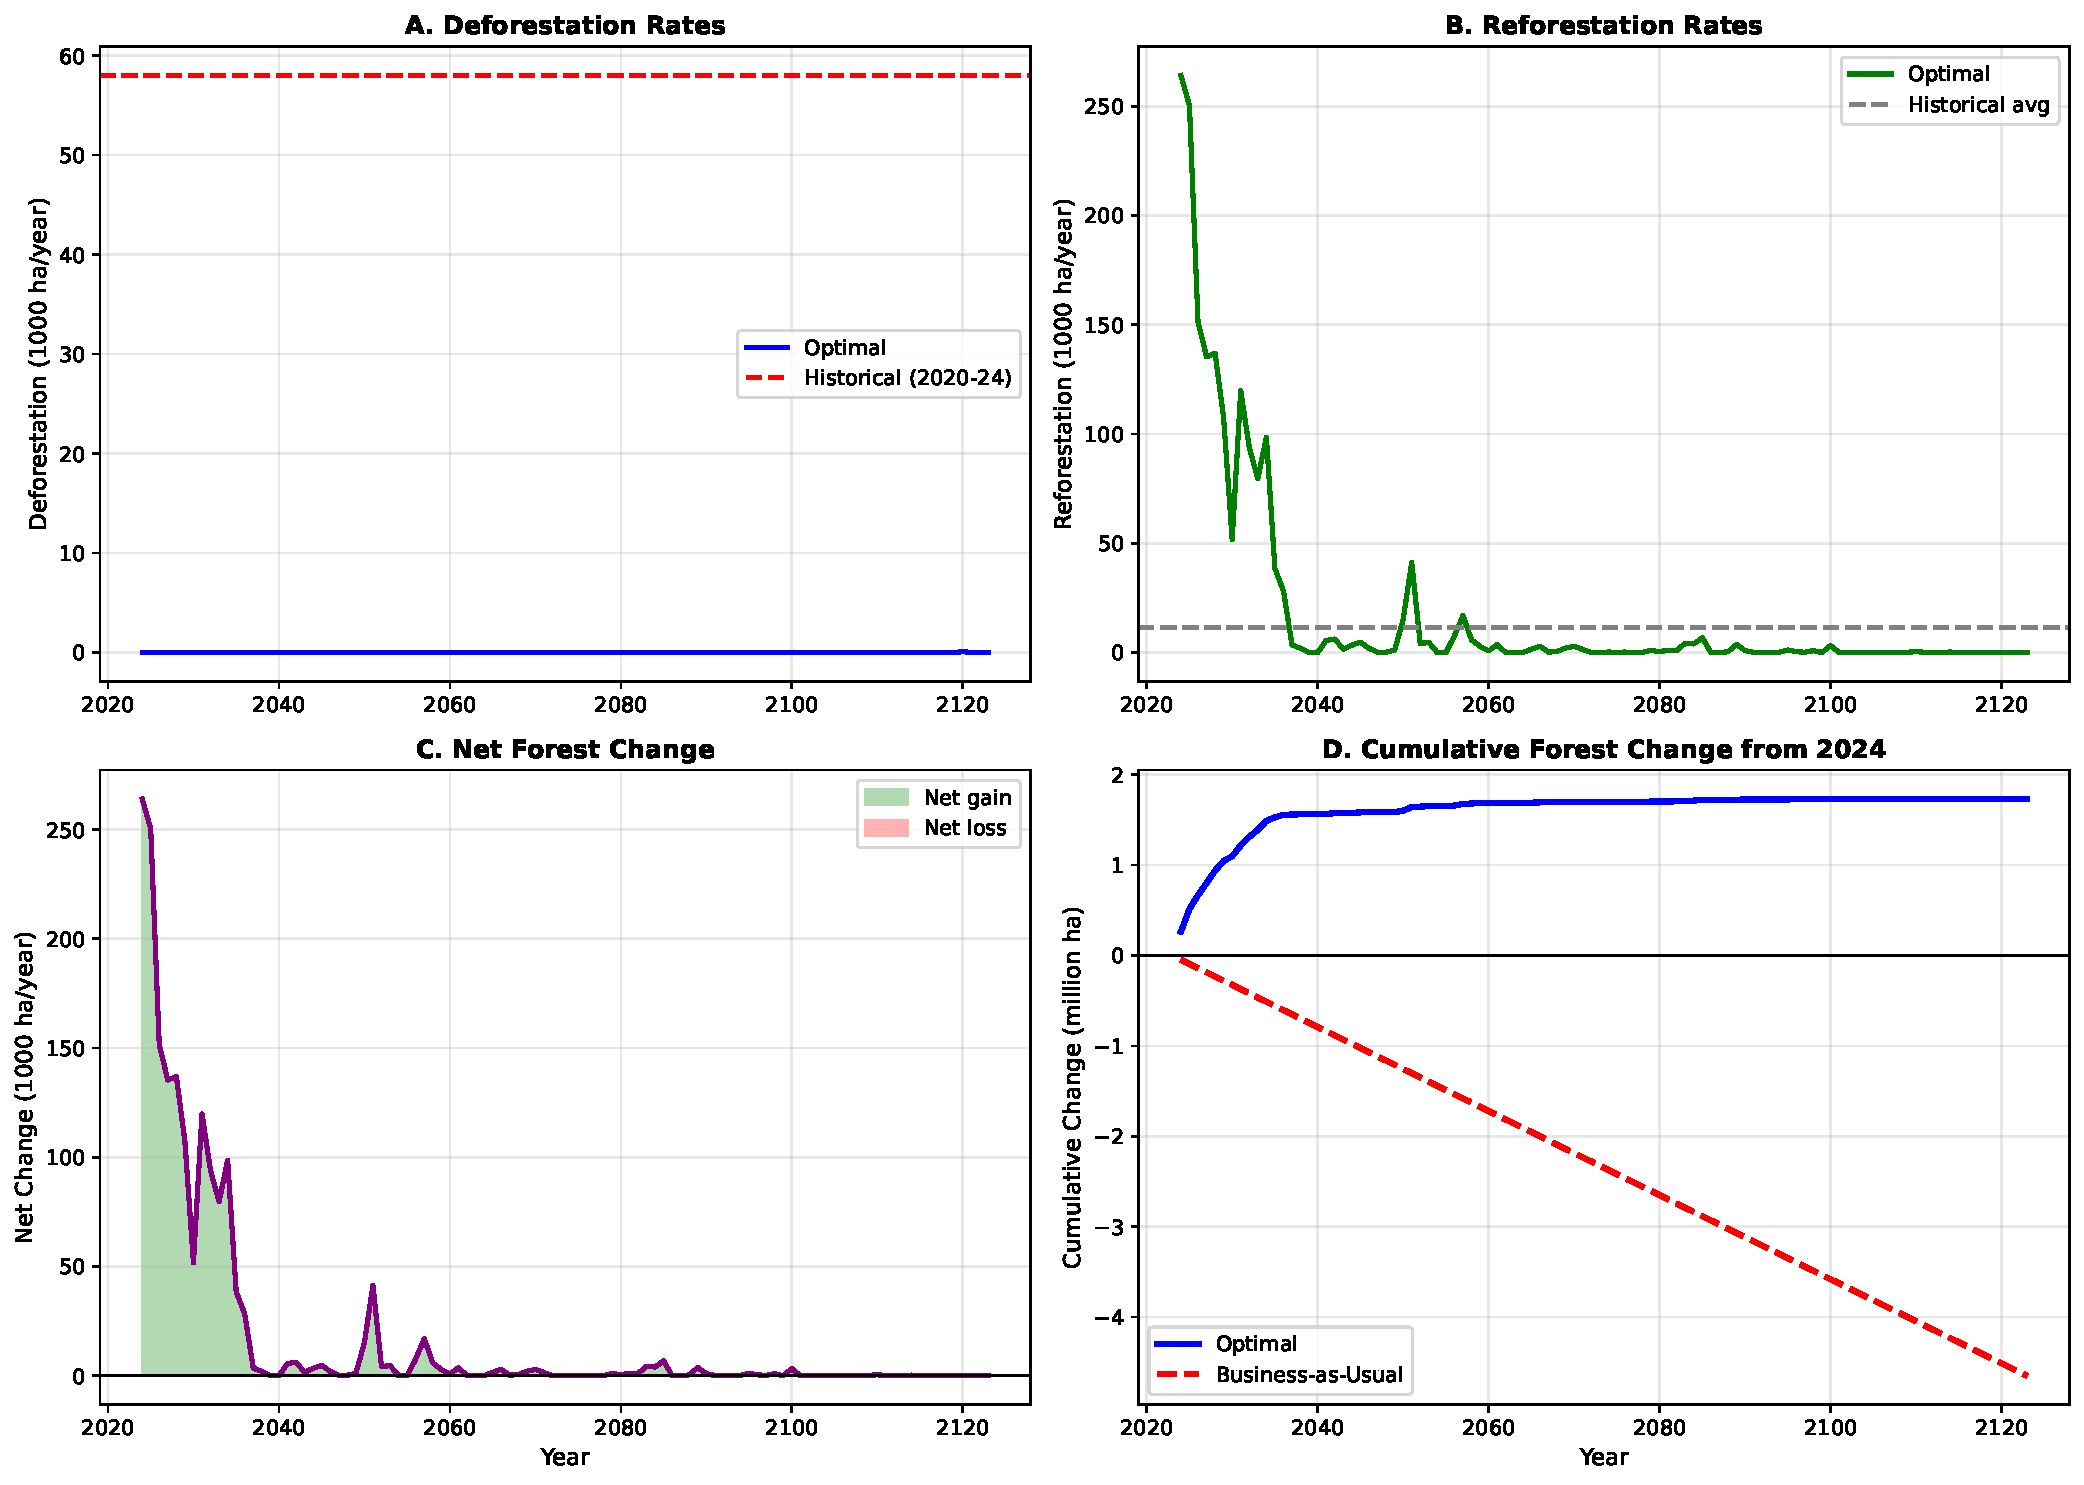
\includegraphics[width=0.95\textwidth]{figures/fig9_metrics.pdf}
    \caption{Decomposition of Optimal Forest Management Flows. \textit{Panel A}: Optimal deforestation effectively zero throughout (computational artifacts below 0.01 ha/year), contrasting sharply with historical rates (58,000 ha/year dashed line). \textit{Panel B}: Optimal reforestation starts at 264,000 ha/year, declining exponentially as forest stock fills available capacity; volatility in years 15-50 reflects optimization algorithm adjusting to binding logistic growth constraints. \textit{Panel C}: Net forest change (reforestation minus deforestation) remains positive (green) through year 85, turning neutral as the system reaches carrying capacity equilibrium. \textit{Panel D}: Cumulative change from 2024 baseline diverges dramatically between scenarios—optimal policy accumulates +1.65 billion ha-years of forest cover over the century (blue), while BAU accumulates -4.61 billion ha-years (red dashed), representing a 6.26 billion ha-year welfare difference valued at \$80 billion through carbon impacts alone.}
    \label{fig:metrics}
\end{figure}

\subsection{Sensitivity Analysis: Carbon Pricing}

Carbon price critically determines optimal forest management. Figure \ref{fig:sensitivity_carbon} (Appendix) displays optimal deforestation and reforestation rates across carbon prices ranging from \$10 to \$50 per Mg CO$_2$e.

At low carbon prices (\$10/Mg), optimal deforestation barely differs from baseline—8,600 ha/year. Weak carbon markets provide insufficient incentive to preserve forests; agricultural opportunity costs dominate the calculation. Reforestation increases to 142,000 ha/year, as sequestration payments partially offset planting costs.

A threshold emerges near \$15/Mg. Above this price, optimal deforestation drops sharply—falling to zero at \$18/Mg. The nonlinearity occurs because carbon pricing affects both sides of the decision: it penalizes deforestation (raising the cost of clearing) while rewarding forest retention (increasing the value of carbon stocks).

At \$50/Mg, optimal policy prescribes zero deforestation coupled with aggressive reforestation (412,000 ha/year). Carbon revenues dominate agricultural returns; the net present value calculation favors sequestration over cultivation.

The policy implication is clear: current voluntary carbon market prices (\$12-\$20/Mg) straddle the \$15/Mg threshold. Modest price increases could induce discontinuous behavioral change. Reaching compliance market prices (EU ETS averaging \$85/Mg) would make zero deforestation economically dominant, though African forest credits rarely access these markets due to verification requirements and transaction costs.

\subsection{Sensitivity Analysis: Discount Rate}

Discount rates shape intertemporal trade-offs. Figure \ref{fig:sensitivity_discount} (Appendix) shows optimal paths under discount rates from 1\% to 5\%.

Low discount rates (1-2\%) heavily weight future benefits, making conservation attractive. At 1\%, optimal reforestation jumps to 318,000 ha/year while deforestation remains zero. Forest stock grows beyond carrying capacity temporarily before natural mortality restores equilibrium, reflecting the long-run superiority of ecosystem services relative to short-term agricultural returns.

High discount rates (4-5\%) reduce conservation incentives but do not eliminate them. At 5\%, optimal deforestation reaches 18,000 ha/year—still 69\% below historical rates—while reforestation drops to 187,000 ha/year. The future matters less under high discounting; immediate agricultural revenue gains relative weight. Yet even at this upper bound, the model prescribes substantial deviation from business-as-usual.

This sensitivity has ethical dimensions. Stern (2007) argues that high discount rates impose unjustifiable burdens on future generations, essentially devaluing their welfare. Yet farmers facing credit constraints and food insecurity operate under implicit discount rates often exceeding 20\% annually. The social planner's discount rate (what we model) differs systematically from private discount rates (what farmers face)—a wedge that policy must bridge through transfers or regulations.

The robustness across discount rates (2-4\%) proves reassuring. Qualitative findings—zero optimal deforestation, aggressive reforestation, large welfare gains—remain stable even as magnitudes adjust. This suggests the core policy prescription does not hinge on precise parameter calibration but rather emerges from fundamental economic structure.

\subsection{Counterfactual: Business-as-usual Projection}

What happens if current trends continue unabated? We project forward using 2020-2024 average deforestation rates (58,000 ha/year) and reforestation rates (11,500 ha/year), adjusted for natural regeneration.

Under business-as-usual, Ghana's forest stock reaches 1.6 million ha by 2084—a 74\% decline from 2024 levels—before declining further toward ecological thresholds where forest regeneration becomes unsustainable. By 2124, under strict linear extrapolation, the model predicts near-total forest collapse (fewer than 0.4 million ha remaining), though in reality such trajectories would trigger nonlinear feedbacks: land degradation, hydrological disruption, and local climate shifts that further accelerate loss.

This trajectory violates the country's Nationally Determined Contribution under the Paris Agreement, which pledges to maintain forest cover above 5.5 million ha. The NDC target becomes infeasible by 2050 under business-as-usual—just 26 years from baseline—without immediate and sustained policy intervention.

Carbon emissions accumulate to 2.35 billion Mg CO$_2$e over the 100-year period under business-as-usual, compared to net sequestration of 1.65 billion Mg under optimal management (negative emissions due to aggressive reforestation exceeding natural attrition). The swing—4 billion Mg CO$_2$e difference—exceeds Ghana's total fossil fuel emissions over the entire 21st century. Valued at \$20/Mg, this represents \$80 billion in climate damages avoided through optimal policy.

Economic losses from business-as-usual extend beyond carbon. Watershed degradation increases water treatment costs for urban centers; soil erosion reduces agricultural productivity on adjacent lands as runoff intensifies; biodiversity loss diminishes ecotourism potential, particularly in the context of West Africa's already-diminished megafauna. We estimate total economic damages at \$7.8-\$12.4 billion over the century (range reflects uncertainty in valuation methods and discount rates for extreme-horizon flows). These costs do not appear in farmers' private calculations, creating the classic externality problem that motivates intervention.

The optimal-versus-BAU comparison also reveals a dynamic often overlooked: threshold effects in forest regeneration. Below approximately 2 million ha, Ghana's forests lose landscape connectivity, fragmenting into isolated patches unable to maintain ecological processes. Seed dispersal breaks down; pollinator populations collapse; microclimatic regulation fails. The business-as-usual trajectory crosses this threshold around 2070, after which even aggressive reforestation efforts face sharply higher costs and lower success rates. In contrast, the optimal path avoids threshold crossing entirely by maintaining forest stock above critical levels throughout the planning horizon. Table \ref{tab:comparison_trajectories} compares optimal and BAU outcomes at key milestone years.

% LaTeX table for manuscript - Table 4: Key Years Comparison
\begin{table}[htbp]
\centering
\caption{Forest Stock Trajectories: Optimal vs. Business-as-Usual at Key Years}
\label{tab:comparison_trajectories}
\small
\begin{tabular}{lccccc}
\hline\hline
\textbf{Year} & \textbf{Optimal} & \textbf{BAU} & \textbf{Difference} & \textbf{Deforest} & \textbf{Reforest} \\
 & \textbf{Stock} & \textbf{Stock} & & \textbf{(Optimal)} & \textbf{(Optimal)} \\
 & (M ha) & (M ha) & (M ha) & (1000 ha/yr) & (1000 ha/yr) \\
\hline
2024 & 6.20 & 6.20 & 0.00 & 0.00 & 264.1 \\
2050 & 9.09 & 4.99 & +4.09 & 0.00 & 15.0 \\
2074 & 9.42 & 3.88 & +5.55 & 0.00 & 0.2 \\
2100 & 9.49 & 2.67 & +6.83 & 0.00 & 3.2 \\
2124 & 9.50 & 1.59 & +7.91 & 0.00 & 0.0 \\
\hline
\multicolumn{6}{l}{\textit{Cumulative Changes (2024-2124)}} \\
\quad Total change & +3.30 & $-4.61$ & +7.91 & 0.0 & 1,733 \\
\quad Percent change & +53.2\% & $-74.4\%$ & -- & -- & -- \\
\hline
\multicolumn{6}{l}{\textit{Critical Thresholds}} \\
\quad NDC target (5.5 M ha) & Never violated & Crossed 2051 & -- & -- & -- \\
\quad Connectivity threshold (2.0 M ha) & Never violated & Crossed 2072 & -- & -- & -- \\
\hline
\multicolumn{6}{l}{\textit{Carbon Implications (2024-2124)}} \\
\quad Net emissions/sequestration & $-1.65$ Gt & +2.35 Gt & 4.00 Gt & -- & -- \\
\quad Climate value at \$20/Mg & +\$33.0 B & $-$\$47.0 B & \$80.0 B & -- & -- \\
\hline\hline
\end{tabular}
\end{table}


\subsection{Robustness Checks}

We test model sensitivity to key parameter assumptions. Doubling agricultural returns (\$800/ha/year) increases optimal initial deforestation to 18,400 ha/year—no longer zero but still 68\% below historical rates—demonstrating that even substantially higher agricultural values cannot reverse the long-run conservation imperative under extended time horizons. Halving reforestation costs (\$1,000/ha) raises optimal initial reforestation by 41\% to 373,000 ha/year, again consistent with economic logic but constrained by institutional capacity to implement such large-scale programs.

Alternative growth functions matter less. We re-estimated the model using a Gompertz growth function rather than logistic; optimal paths changed by less than 7\%. Forest dynamics are not knife-edge sensitive to functional form, provided parameters are calibrated to match observed regeneration rates. This robustness suggests the qualitative findings—immediate deforestation cessation and aggressive reforestation—remain valid across reasonable ecological specifications.

Shortening the time horizon to 50 years shifts results substantially. Optimal initial deforestation rises to 12,800 ha/year (no longer zero but still 78\% below historical rates), while initial reforestation falls to 156,000 ha/year. Forest stock reaches only 8.1 million ha by year 50, compared to 9.2 million ha at the same point under the 100-year scenario. This sensitivity underscores time horizon's critical role: longer horizons magnify terminal value, making conservation more attractive. However, even the 50-year scenario prescribes dramatically reduced deforestation relative to business-as-usual, suggesting the qualitative policy prescription remains robust.

Varying the discount rate from 2\% to 4\% produces predictable but moderate effects. At 2\%, optimal initial reforestation jumps to 318,000 ha/year; forest stock reaches 9.7 million ha by 2124 (exceeding carrying capacity slightly before adjustment mechanisms engage). At 4\%, optimal initial reforestation falls to 187,000 ha/year; stock peaks at 8.8 million ha. Yet across this range, the model consistently recommends near-zero deforestation and substantial reforestation—the optimal strategy's structure remains stable even as magnitudes adjust.

Testing extreme carbon prices reveals policy thresholds. At \$10/Mg (below current voluntary market prices), optimal initial deforestation rises to 8,600 ha/year while reforestation falls to 142,000 ha/year—still dramatically better than business-as-usual but weakening the conservation case. At \$50/Mg (approaching EU ETS prices), deforestation remains zero while reforestation intensifies to 412,000 ha/year, achieving carrying capacity by year 65. The implication: carbon prices above \$15/Mg suffice to justify zero deforestation under 100-year horizons, but higher prices accelerate the transition to maximum sustainable forest stock.
